\documentclass[12pt]{article}
\linespread{2.0}
\usepackage{indentfirst}
\usepackage{underscore}
\usepackage{amsmath}
\usepackage{graphicx}
\usepackage{url}
\title{The Prediction of Covid-19 Inpatient Cases with Different Epidemic Prevention Policy}
\author{Donglai Lyu}
\date{\today}
\begin{document}
\maketitle
	\clearpage
	\section{Introduction}
	
	At the end of 2019, Covid-19 has outbreak around the world. Many people's work and lives have been affected by Covid-19, and it is also a huge challenge for the Health Care System in each country. According to the World Health Organization Coronavirus Dashboard \cite{1}, until November 17, 2022, it has 633,263,617 cumulative cases, and 6,594,491 cumulative deaths around the world. Covid-19 continues to impact healthcare systems in various countries, to avoid medical crash, it is important to do the prediction research for Covid-19 inpatient cases. That can help healthcare system to prepare enough medical resources for patients. Also, the prediction research can show the impact of epidemic prevention policy on the number of inpatient people.
	
	It has been almost three years since the Covid-19 outbreak, but the rate of growth in the number of confirmed Covid19 cases has not decreased. on the one hand, as the economic needs for each government and the need for people to get back to normal life have grown stronger and stronger, more and more countries opened the border to allow people to enter. On the other hand, the coronavirus is keeping mutating, and its contagiousness has been getting stronger. Due to those two reasons, doing the prediction for the Covid-19 inpatient cases is very important especially in the period that most countries and regions choose to reopen the border. 
	
	In this paper, I use the Logistic model to do the prediction of inpatient people base on the data from the Google Covid-19 data set. I do research for inpatient cases in the United States and the Hong Kong SAR. Form the existing data, we can get the prediction data, and from this data, we can learn the impact of epidemic prevention policies on confirmed cases in different regions.
	
	\section{Data Description}
	The source for this project is form the Google Covid-19 Open Data \cite{2}. Google Covid-19 Open data is a great source for the research. It includes many aspects such as search trends, vaccination, and hospitalization for the Covid-19 data around the world, and it is wildly use. In this project, I choose the hospitalization data from the Google Covid-19 Open Data as the primary data.
	
	The hospitalization data contains 11 categories. The first category is the date. This category records the date of the daily change in the number of hospitalizations. The second category is the location key, this category records the location of the inpatient cases. The next category is the new hospitalized patients, this category records the number of new hospitalized patients every day. The next category is the cumulative hospitalized patients, this category records the number of total hospitalized patients every day. The next category is the current hospitalized patients, this category records the number of current inpatients cases every day. The next category is the new intensive care patients, this category records the number of new hospitalized patients in ICU every day. The next category is the cumulative intensive hospitalized patients, this category records the number of total hospitalized patients in ICU every day. The next category is the current hospitalized patients, this category records the number of current inpatients cases in ICU every day. The last three category is recording the new, current, and total inpatient cases that use the ventilators in hospital.
	
	This database collects 34 countries and regions inpatients data around the world, this includes Argentina, Australia, and Belgium. For all the countries and regions on the list, I decide to choose United State and Hong Kong SAR. as the location to study in this project. According to Travel States Gov \cite{3}, after June 12, 2022, at 12:01AM ET, entering US border do not need to provide negative Covid-19 test. That means there is no Covid check for entering the US border. Also, Hong Kong released the ``0+3" entry policy for the Covid-19 on September 26, 2022 \cite{4}. Although there is no quarantine required to enter Hong Kong, but the government in Hong Kong SAR still monitoring the Covid cases on the border. Comparing with United State, Hong Kong government has stricter control over the Covid outbreak, and this is the reason why choosing these two locations as the research data. For the inpatient cases data, I choose the category of cumulative hospitalized patients, because this category records all the inpatients cases that we need to use, and this data is the most complete of all categories.
	
	For the implementation, I use Python to optimize the database. The original database is an csv form. I use the function ``file = file[file[`location_key'].isin([``US"])]" and ``file2 = file2[file2[`location_key'].isin([``HK"])]" to find all US and HK inpatient cases data form the original data. Then, I use the ``file.drop" function to drop all other categories beside the category of cumulative hospitalized patients. After that, I created two csv form to store the completed processing data separately. The completed processing data only contains date, location key, and cumulative hospitalized patients. The complete processing form is ``US_hospitalizations.csv" and ``HK_hospitalizations.csv".
	\section{Math Model Description}
	For the math model description, I choose logistic model. According to the Wikipedia \cite{5}, logistic regression is used in various fields, including machine learning, most medical fields, and social sciences. For example, the Trauma and Injury Severity Score , which is widely used to predict mortality in injured patients. Many other medical scales used to assess severity of a patient have been developed using logistic regression. Logistic regression may be used to predict the risk of developing a given disease, based on observed characteristics of the patient. So, Using the logistic model to predict the Covid inpatient cases is appropriately. The formula shows below is commonly used for this model \cite{6}:
	\[ y=\frac{K}{1+be^{-ax} } ,a>0,b>0\]
	\noindent
	For this model, use this formula to predict cases and we can get:
	\[ y=K/(1+b*exp(-at)),a>0,b>0\]
	\noindent
	In the above formula, y as cumulative hospitalized patients for each day, t as the date, K as the maximum number of cumulative inpatient cases. The a and b are the parameters controlling the speed of infection.
	
	For the implementation, I use python to do the prediction. The code shows below is the implementation for the formula shows above. For the parameters, I set t as time, t0 as initial time, P0 is initial value, K as capacity, and r is increase rate.
	\begin{figure}[h]
		\centering
		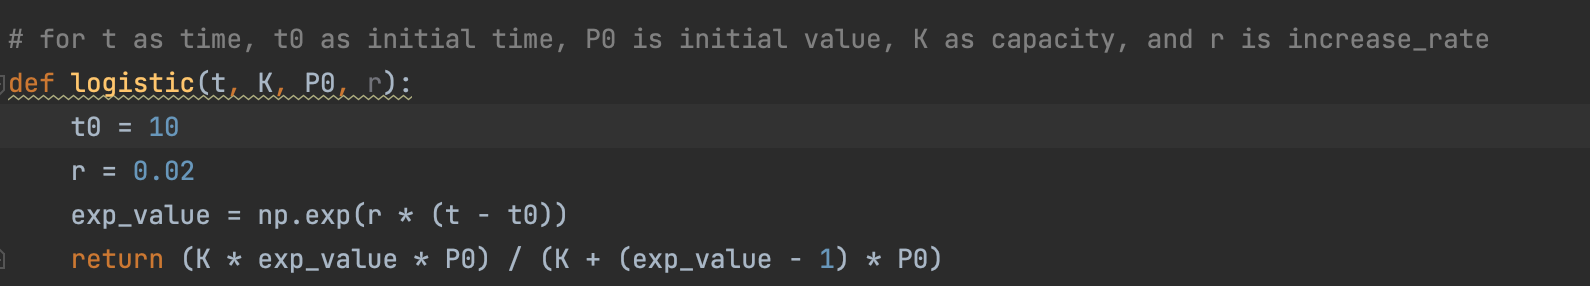
\includegraphics[width=1\textwidth]{Figure1.png}
		\caption{Code}
	\end{figure}
	
	\section{Model Prediction}
	For the model prediction part, I use the logistic model to predict the Covid inpatient cases in United States and Hong Kong SAR. First of all, I tested whether the model is reliable. I randomly picked 11 data from March 10, 2020, to March 25, 2020, in “US_hospitalizations.csv”. Then I import that data to run the prediction model. By adjusting the value of parameter r, it is found that a value of r around 0.45 gives a curve that better matches the number of Covid hospitalizations in the United States from March to April (As figure 2 shows above).
	\begin{figure}[h]
		\centering
		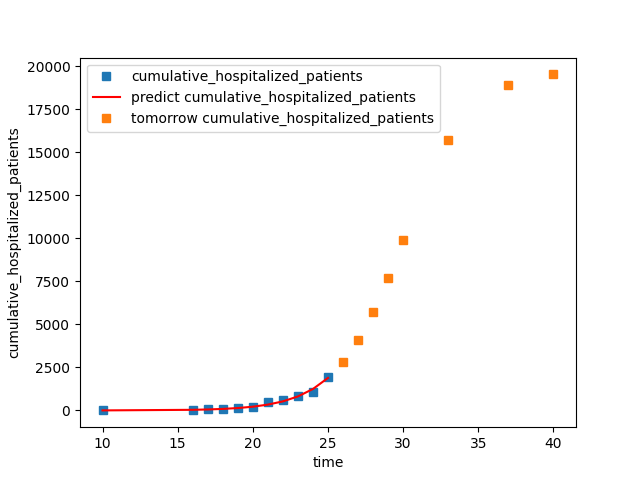
\includegraphics[width=0.8\textwidth]{Figure2.png}
		\caption{Prediction for Hospitalization in the US for 1 Month}
	\end{figure}
	
	As the initial date is March 10, 2022, then the time value is 40, that means the date of the time values shows is April 10, 2022. At that date, the predict value of the cumulative hospitalized patients is around 20,000 and the real value of the cumulative hospitalized patients in April 10 in United State is 18,923. The predict cases is very close to real cases, that means using this model to predict the inpatient cases is reliable.
	
	Then apply this model to do the prediction for the cumulative hospitalized patients’ cases in United States base on the dataset that been processed before. Set the initial time t0 as 10, when the increase rate r equal to 0.0061, the curve is better matches the number of Covid hospitalizations in the United States. (Predict figure 3 shows below)
	
	\begin{figure}[h]
		\centering
		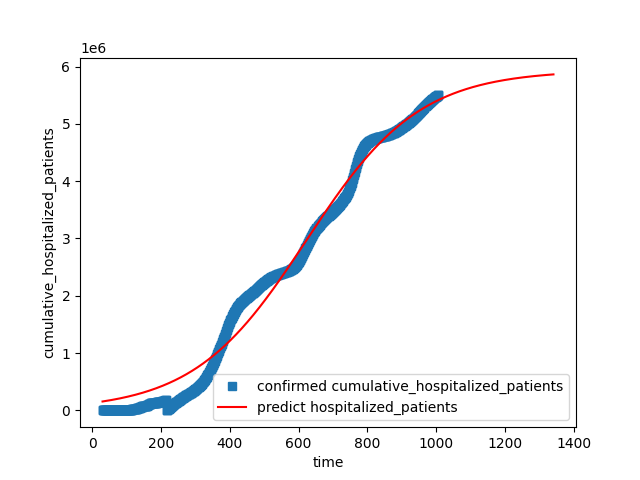
\includegraphics[width=0.8\textwidth]{Figure3.png}
		\caption{Prediction for Hospitalization in the US}
	\end{figure}
	
	Also, apply logistic model to do the prediction for the cumulative hospitalized patients’ cases in Hong Kong SAR base on the dataset that been processed before. Set the initial time t0 as 10, when the increase rate r equal to 0.02, the curve is better matches the number of Covid hospitalizations in the Hong Kong SAR. (Predict figure 4 shows below)
	\clearpage
	\begin{figure}[h]
		\centering
		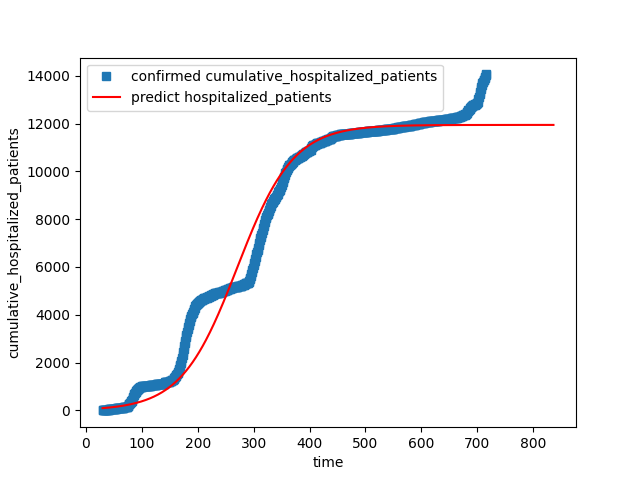
\includegraphics[width=0.8\textwidth]{Figure4.png}
		\caption{Prediction for Hospitalization in Hong Kong SAR}
	\end{figure}
	
	Form the inpatient cases data in Hong Kong SAR, there are two there are two clear points of inflection appears in the time value around 150 and around 300. So, I decide to divide the data into three parts based on those two points and check the increase rate r value of each part separately.
	
	For the first part, I check the data from January 23, 2020, to the June 30, 2020. This data is in the early stage for the Covin-19 outbreak. In this period, the initial time t0 is set as 10 and when the increase rate r equal to 0.069, the curve is better matches the number of Covid hospitalizations in the Hong Kong SAR(figure 5 shows below).
	\clearpage
	\begin{figure}[h]
		\centering
		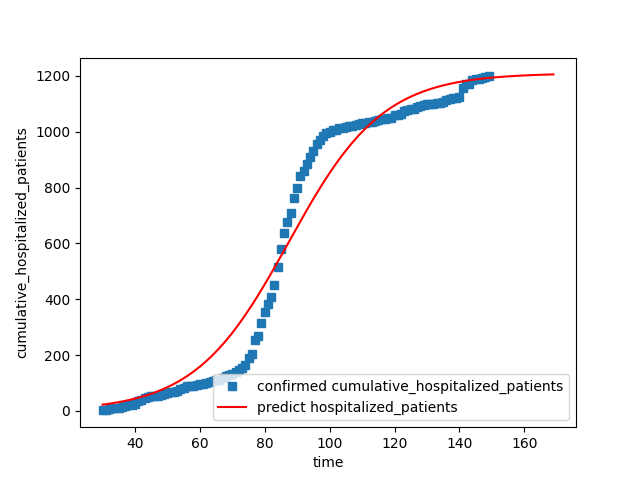
\includegraphics[width=0.8\textwidth]{Figure5.png}
		\caption{Prediction for Hospitalization in Hong Kong SAR Part1}
	\end{figure}

	For the second part, I check the data from July 1, 2020, to the November 1, 2020. This data is in the middle stage for the Covin-19 outbreak. In this period, the initial time t0 is set as 10 and when the increase rate r equal to 0.06, the curve is better matches the number of Covid hospitalizations in the Hong Kong SAR(figure 6 shows below).
	\clearpage
	\begin{figure}[h]
		\centering
		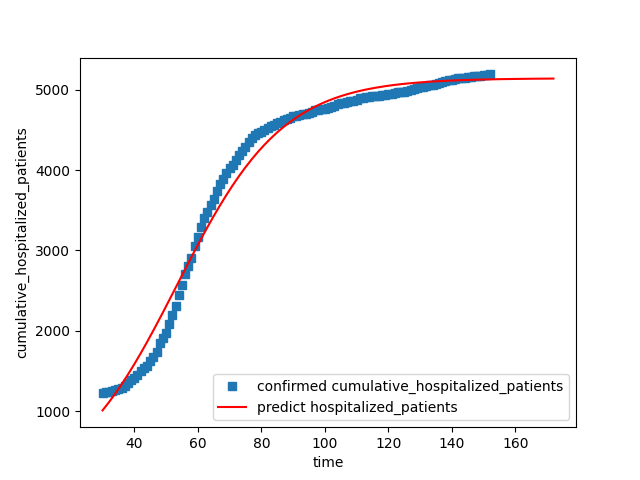
\includegraphics[width=0.8\textwidth]{Figure6.png}
		\caption{Prediction for Hospitalization in Hong Kong SAR Part2}
	\end{figure}
	
	For the third part, I check the data from November 1, 2020, to the January 1, 2022. This data is in the late stage for the Covin-19 outbreak. In this period, the initial time t0 is set as 10 and when the increase rate r equal to 0.02, the curve is better matches the number of Covid hospitalizations in the Hong Kong SAR(figure 7 shows below).
	\clearpage
	\begin{figure}[h]
		\centering
		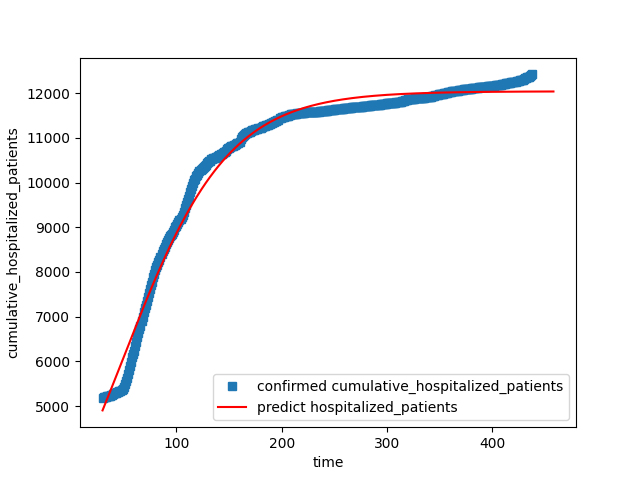
\includegraphics[width=0.8\textwidth]{Figure7.png}
		\caption{Prediction for Hospitalization in Hong Kong SAR Part3}
	\end{figure}
	
	\section{Discussion}
	
	In this prediction, we need to adjust the increase rate value r to make curve better matches the data number of the Covid hospitalizations. In pervious prediction, we found that the increase rate value r of the Unite States is 0.0061 and the increase rate value r of Hong Kong SAR is 0.02. The increase rate value can show how effective a place is in controlling the epidemic, when the r value of a place is higher, it means that this place is better at controlling the epidemic. Form above data, we can see that Hong Kong SAR is doing better on controlling the Covid-19 outbreak. It is true because Hong Kong SAR has stricter controls on the new coronavirus outbreak than the United States. As time gets longer, we can also see from the decrease of the Hong Kong's r value that Hong Kong's Anti-epidemic measures are being reduced step by step.
	Form the prediction data above, it is easy to tell that the total inpatient data of Covid-19 in the United State will close to 6 million in the following year, and the total inpatient data of Covid-19 in Hong Kong SAR will close to 12,000 in the following 150 days. Fortunately, according to prediction, the cumulative number of Covid-19 inpatient cases in both United States and Hong Kong SAR will only increase slowly for some time afterwards.
	\clearpage
	\section*{Reference}
	\begin{thebibliography}{99}
		
		\bibitem[2022]{1}
	World Health Organization.
	\newblock WHO Coronavirus (COVID-19) Dashboard.
	\newblock 2022.
	\newblock Available from: \url{https://covid19.who.int}.
	
	\bibitem[2022]{2}
	Google.
	\newblock Covid-19 Open Data.
	\newblock 2022.
	\newblock Available from: \url{https://github.com/GoogleCloudPlatform/covid-19-open-data/blob/main/docs/table-hospitalizations.md}.
	
	\bibitem[2022]{3}
	Travel.State.Gov.
	\newblock COVID-19 Testing Order Rescinded.
	\newblock 2022.
	\newblock Available from: \url{https://travel.state.gov/content/travel/en/international-travel/before-you-go/covid-19_testing_required_US_Entry.html}.
	
	\bibitem[NDTV(2022)]{4}
	NDTV.
	\newblock Hong Kong Scraps Mandatory Quarantine For International Travellers With New ``0+3" Rule.
	\newblock 2022.
	\newblock Available from: \url{https://www.ndtv.com/world-news/hong-kong-scraps-mandatory-quarantine-for-international-\\travellers-with-new-0-3-rule-3372704}.
	
	\bibitem[2022]{5}
	Wikipedia.
	\newblock Logistic regression.
	\newblock 2022.
	\newblock Available from: \url{https://en.wikipedia.org/wiki/Logistic_regression}.
	
	
	\bibitem[2020]{6}
	Zhihu.
	\newblock Prediction of 2019 Novel Coronavirus (2019-nCOV) Outbreak Based on Logistic Growth Curve Model.
	\newblock 2020.
	\newblock Available from: \url{https://en.wikipedia.org/wiki/Logistic_regression}.
		
	\end{thebibliography}



\end{document}
